%%%%%%%%%%%%%%%%%%%%%%%%%%%%%% -*- Mode: Latex -*- %%%%%%%%%%%%%%%%%%%%%%%%%%%%
%% 10-07-system.tex --  HICSS 44 Kukui Cup paper
%% Author          : Philip Johnson
%% Created On      : Mon Sep 23 11:52:28 2002
%% Last Modified By: Philip Johnson
%% Last Modified On: Fri Jun 11 16:21:03 2010
%%%%%%%%%%%%%%%%%%%%%%%%%%%%%%%%%%%%%%%%%%%%%%%%%%%%%%%%%%%%%%%%%%%%%%%%%%%%%%%
%%   Copyright (C) 2009 Philip Johnson
%%%%%%%%%%%%%%%%%%%%%%%%%%%%%%%%%%%%%%%%%%%%%%%%%%%%%%%%%%%%%%%%%%%%%%%%%%%%%%%
%% 

\section{System Design}
\label{sec:system-design}

\subsection{Requirements}

As our related work findings illustrate, current software for energy
competitions tends to be either commercial, closed systems, or special
purpose, ``on-off'' systems.  We strive in this project to create
software with an architecture that is open, extensible, and easily tailored
to the needs of different universities.  We intend the software
infrastructure from this project to provide as much of a research
contribution as our actual experimental results.

The following general requirements inform our system design.

{\em Open source.}  To maximize the potential for community
participation in development as well as use of the software, we make
all components available as open source, and utilize only freely
available third party components for development.  There are no software
costs associated with the use of our system.

{\em Platform, language, and meter neutrality.}  We want to avoid lock-in
to any particular platform, language, or metering technology.  To avoid
platform lock-in, we develop all components using technologies such as
Java, Python, Javascript, and Google Visualizations that are available on
Windows, Macintosh, and Linux platforms.  To avoid language lock-in, the
system observes a service-oriented architecture, where components
communicate with each other over HTTP via a RESTful API.  This isolates
language dependencies to individual services.  For example, the WattDepot
server is written in Java, while the Makahiki web application framework is
written in Python.  Finally, to avoid metering technology lock-in, the
system architecture involves ``sensors'' that query any given meter using
its native protocol, then translates that into a common format for use in
the rest of the system.  Thus, adapting the system to a new meter
technology simply involves implementing the sensor for that technology.

{\em Feature subsetting.} Not all universities need or want the same 
level of sophistication in their dorm energy competitions.  In reviewing 
other sites, we found that they ranged from simple single web pages that are 
edited manually, to advanced sites that integrate near-real time energy data. 
Our software is designed to support users with a variety of needs. 

\subsection{Architecture}

\begin{figure*}[!th]
  \center
  \includegraphics[width=0.8\textwidth]{architecture.eps}
  \caption{\em \small System Architecture: Dorm energy usage is captured by one or more meters, which 
are queried by WattDepot sensors and the raw data sent to the WattDepot server. Analyses are computed
and stored in cloud-based services for ease of retrieval and display in the Makahiki web application.}
  \label{fig:architecture}
\end{figure*} 

Figure \ref{fig:architecture} illustrates the high-level architecture of
the system. There are three basic subsystems in this architecture.  The
first is the dorm electrical infrastructure, illustrated on the left hand
side of the diagram.  This infrastucture includes power distribution to
dorm rooms where residents consume power.  It also includes one or more
electrical meters that monitor power consumption and that are connected to
the Internet.  The second subsystem is WattDepot, an open source suite of
tools we have developed for enterprise-level collection, storage, analysis,
and presentation of energy data.The third subsystem is Makahiki, an open
source framework for building dorm energy competition web applications.
The following sections discuss each of these architectural components in
more detail.

\subsubsection{WattDepot Sensors}

Electricity can be generated and/or consumed by a wide variety of devices
and monitored by a wide variety of metering technologies.  Many energy
management software systems are tied to a particular energy device and/or
meter; indeed, they are often marketed as an accessory to the hardware.
For example, most commercial energy meter manufacturers provide software
for storing data about the power generated by the meter and simple
visualizations of the power generated over time.

Our architecture attempts to make the software as independent from
the energy hardware devices as possible.  To achieve this independence, the
WattDepot architecture includes ``sensors'', or small software processes
that query any given energy device according to its native protocol,
collect standard information, and then send it to a WattDepot server using
the Internet and the RESTful WattDepot API over HTTP.  This design means
that new energy devices can be integrated easily into the WattDepot
software ecosystem just by writing the sensor interface.  The use of a
RESTful HTTP protocol for communication with the WattDepot server means
that the sensor can be implemented in any programming language.

We have implemented WattDepot sensors for the TED 5000 home energy device, 
the Veris power meter collected through the Building Manager Online system,
and for the Acuvim and Shark commercial energy meters. The latter sensors
are based upon the standard ModBus/TCP protocol. 

Sensors transmit data to a WattDepot server using a standardized, published
protocol, as discussed next.

\subsubsection{WattDepot Server}

A WattDepot server accepts raw energy data from devices (via sensors) and
makes this data (or analyses based upon it) available to clients.  The
WattDepot server implements a variety of design decisions intended to
improve its generality, reusability, and extensibility, including: (1) a
RESTful API, (2) a pluggable back-end database, (3) aggregation via
``virtual'' sources, (4) data interpolation, and (5) multiple
representations.

{\em RESTful API.} WattDepot conforms to modern web service design best
practices by providing a RESTful API.  REST (REpresentational State
Transfer) \cite{REST} is a specification paradigm, which, when applied to
web services, generally results in more easily usable and extensible
communication than alternatives such as SOAP. The details of RESTful design
are beyond the scope of this paper. Some of the implications include
URLs that can serve as unique identifiers for energy data and the use of HTTP
methods such as PUT, POST, GET, and DELETE to add, amend, retrieve, and
delete energy data. The WattDepot API \cite{WattDepotAPI} provides more
details and a full specification of the supported operations.

{\em Pluggable back-end database.} The WattDepot server implements an
abstraction layer that enables the server to be built with a variety of
different persistence mechanisms.  By default, WattDepot uses the Apache
Derby relational database, which is a high performance, embedded database
written in Java.  However, WattDepot can be ported to other relational or
non-relational database systems by implementing an interface and setting some 
run-time configuration parameters. 

{\em Aggregation via virtual sources.} The data from a single physical
meter is generally represented in WattDepot as a ``Source''.  Each
WattDepot Source can indicate the power generated or consumed by that
device at any moment in time, the energy generated or consumed by that
device over a period of time, the carbon intensity associated with that
device, and other features.  In addition to this one-to-one correspondence,
WattDepot also supports the definition of ``virtual'' Sources, which are
Sources defined as the aggregation of other Sources.  For example, a floor
on a building might have two meters collecting energy consumption data for
the two sections of the floor.  WattDepot allows users to
define a virtual Source representing the aggregation of the data stream
from the two meters.  This virtual Source thus represents the total energy
consumption for the floor. Virtual Sources can be arranged in a hierarchy,
such that the virtual Sources for each floor in the building can themselves
be contained in a virtual Source representing the entire building's energy
consumption.

{\em Data interpolation.} One common initial roadblock to analyzing energy
data collected from multiple sources is the ``timestamp problem''. For
example, assume that energy consumption on a building floor is collected by
two meters, and that energy data is collected from those meters becomes
available approximately every 15 minutes, but the timestamps associated
with the data for a given time period differ by a minute or two.
Determining the aggregate energy consumption is no longer a simple matter
of importing the two data sets into a spreadsheet and using a summation
macro, because the timestamps from the two meters do not ``match up''.
WattDepot addresses this problem by providing automatic interpolation. For
example, assume a meter sent energy data at roughly 30 minute intervals:
11:23 AM, 11:56 AM, 12:25 PM, and 1:01 PM.  You can request the energy consumed
by this Source between 12:00 PM and 1:00 PM, for example, and WattDepot will
automatically interpolate the raw data values to provide an estimate for
the interval of interest.  Automatic linear interpolation enables virtual Sources
to return reasonable values even when its constituent Sources send data at
different times and with different frequencies. 

{\em Multiple representations.} One benefit of a RESTful architecture is
the separation of a ``resource'' from its ``representation''.  In
WattDepot, this separation means that data and analyses for a given Source can
be provided in different ways, depending upon the needs of the client.  So
far, WattDepot can provide data to clients using XML, JSON (the format
supported by Google Visualizations), and CSV (comma-separated values),
which is useful for importing WattDepot data into other tools for
additional analysis.

\subsubsection{WattDepot Cloud Cache}

A typical dorm energy competition will involve hundreds to thousands of
students.  Energy data requests are characterized by the desire for
relatively recent results (for example, how much power did my dorm use in
the last hour, and how does that compare to usage during the same hour over
the past month?) and the fact that those results do not tend to be
user-specific (monitoring the energy usage of individual dorm members is
not practical at the current time; the most fine-grained collection we have
seen is floor-level). These two application characteristics argue for
caching of results so that the WattDepot server is not processing the same
request hundreds of times.

An architectural question is where that cache of reusable data should be
placed.  There are three choices: in the server, in the web application, or
in some other service ``in between'' the server and the web application.
All of these approaches have their strengths and weaknesses.  Our system
architecture chooses the last approach, in which a service called
WattDepot-GData creates Google Doc spreadsheets containing high level
abstractions of the raw data stored in the WattDepot server.  We chose the
Google Doc cloud-based storage system because it is free, it is scalable
and very high performance, and it integrates extremely well with the Google
Visualization API.  This latter feature enables the Makahiki web
application framework to provide advanced, interactive visualizations of
energy data with very little end-user coding.

\subsubsection{Makahiki}

\begin{figure*}[!th]
  \center
  \includegraphics[width=0.8\textwidth]{makahiki.eps}
  \caption{\em \small An example dorm energy web application built with Makahiki.}
  \label{fig:makahiki}
\end{figure*} 

The final subsystem in our architecture is called Makahiki, which is a
framework for developing dorm energy competition web applications.  Figure
\ref{fig:makahiki} illustrates the home page for the University of Hawaii
dorm energy web application built as a configuration of Makahiki. As a
framework, Makahiki supports several forms of tailoring without requiring
any editing of the underlying Python source code.

{\em Configurable look and feel.} The color scheme and logos for the site
are defined in CSS files that can be edited or replaced to best reflect the
University's color scheme. At the University of Hawaii, Makahiki is
configured with a green and white color scheme and the ``Kukui Cup'' name
and logo.   We use the JQuery ThemeRoller appplication to simplify the generation of 
alternative look and feels.

{\em Configurable display panes.} Each page in the web application generated by Makahiki
contains a number of display panes. The contents of these display panes can be easily 
reconfigured. For example, the form of energy visualization can be changed by editing 
the underlying Javascript associated with the display pane. 

{\em Configurable functional modes.}  Makahiki supports several functional ``modes'', which 
enable it to conform to the needs of a wide variety of dorm energy competitions.  

The ``single page'' mode is the simplest mode, which enables a university
to create a simple, single page website with a matching look and feel for
their university.  In single page mode, energy data and dorm standings can
be visualized by manually creating Google Doc spreadsheets and configuring
the display panes to visualize the data as tables or bar charts.  In this
basic functional mode, there need not be any use of WattDepot; all data can
be collected manually by competition organizers and entered into
spreadsheets for display.

In ``multi page'' mode, Makahiki generates a web application containing a
Home page, a Resources page, an Energy data page, a Competition page, and
an About page.  Multi page mode provides a more comprehensive web
application that enables the university to provide significantly more
information than is possible with single page mode.  As with single page
mode, multi page mode does not require WattDepot.

The final mode is called ``login'' mode, and it is in this mode that
Makahiki provides features not currently found in other dorm energy
competition web applications.  In this mode, each resident of the dorm can
login to their own personally customized home page, and enables a set of
behavioral change tools including activities, commitments, goals, and a
parallel competition based upon a point system for engaging with these
tools.  Login mode requires automated access to energy data and so
WattDepot is required.  Figure \ref{fig:makahiki-login} illustrates a sample
configuration of the individual user home page. 

\begin{figure*}[!th]
  \center
  \includegraphics[width=0.8\textwidth]{makahiki.login.eps}
  \caption{\em \small The personalized user home page with floor-level monitoring and behavioral change tools 
including commitments, activities, and goals.}
  \label{fig:makahiki-login}
\end{figure*} 




















